% ------------------------------------------------------------------------------
% TYPO3 Version 10.1 - What's New (French Version)
%
% @license	Creative Commons BY-NC-SA 3.0
% @link		http://typo3.org/download/release-notes/whats-new/
% @language	French
% ------------------------------------------------------------------------------

\section{Interface Utilisateur Backend}
\begin{frame}[fragile]
	\frametitle{Interface Utilisateur Backend}

	\begin{center}\huge{Chapitre 1~:}\end{center}
	\begin{center}\huge{\color{typo3darkgrey}\textbf{Interface Utilisateur Backend}}\end{center}

\end{frame}

% ------------------------------------------------------------------------------
% Feature | 89115 | Auto slug update and redirect creation on slug change

\begin{frame}[fragile]
	\frametitle{Interface Utilisateur Backend}
	\framesubtitle{Mise à jour des slugs et des redirections (1)}

	\begin{itemize}
		\item Lorsque les utilisateurs changent le chemin d'URL d'une page (le Slug),
			l'ancienne URL devient inaccessible.
		\item Cela peut générer une erreur «~page non trouvée~» sur la page,
			impactant les URL de ses sous-pages.
	\end{itemize}

	\begin{figure}
		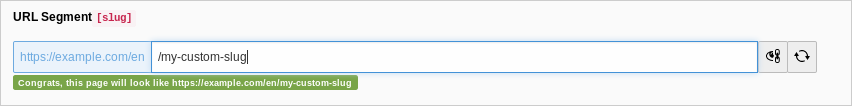
\includegraphics[width=0.80\linewidth]{BackendUserInterface/89115b-AutoSlugUpdateAndRedirectCreationOnSlugChange.png}
	\end{figure}

	\begin{itemize}
		\item Depuis TYPO3 v10.1, deux actions permettent d'éviter cette erreur~:

			\begin{itemize}
				\item Les slugs des sous-pages sont mises à jour automatiquement
				\item Des redirections de l'ancienne à la nouvelle URL sont créées
			\end{itemize}

	\end{itemize}

\end{frame}

% ------------------------------------------------------------------------------
% Feature | 89115 | Auto slug update and redirect creation on slug change

\begin{frame}[fragile]
	\frametitle{Interface Utilisateur Backend}
	\framesubtitle{Mise à jour des slugs et des redirections (2)}

	\begin{itemize}
		\item Les utilisateurs Backend sont informés de ces actions et peuvent
			facilement revenir en arrière en un clic~:

	\end{itemize}

	\begin{figure}
		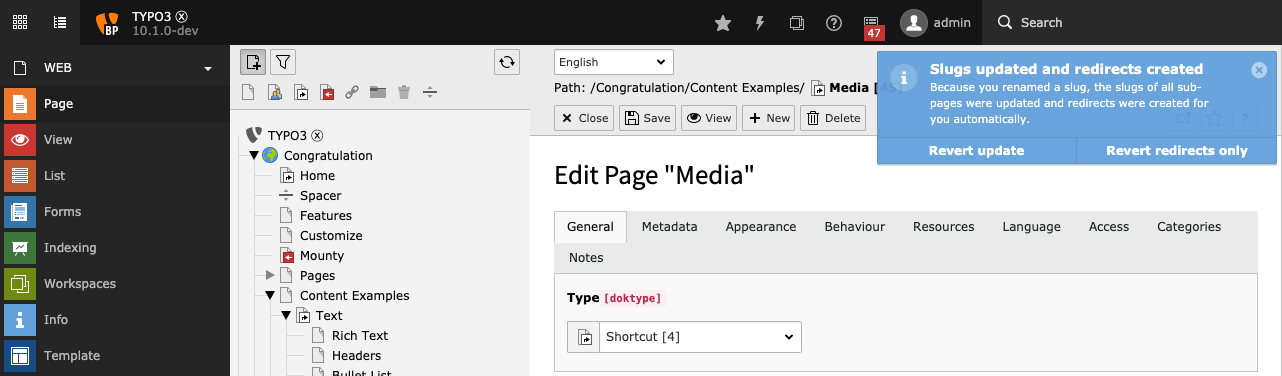
\includegraphics[width=0.80\linewidth]{BackendUserInterface/89115c-AutoSlugUpdateAndRedirectCreationOnSlugChange.png}
	\end{figure}

\end{frame}

% ------------------------------------------------------------------------------
% Feature | 85918 | Hide in menu / Show in menu entry for pages in context menu

\begin{frame}[fragile]
	\frametitle{Interface Utilisateur Backend}
	\framesubtitle{Afficher/masquer dans le menu}

	Une nouvelle entrée est ajoutée au menu contextuel pour afficher/masquer les pages.

	\begin{figure}
		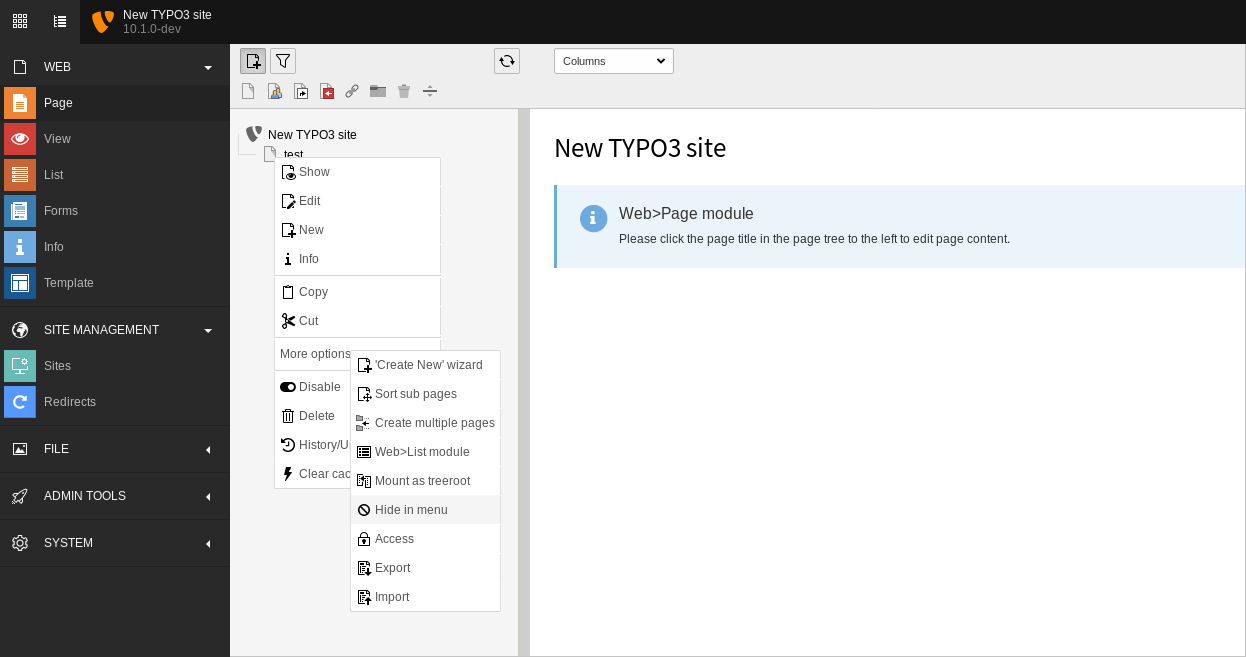
\includegraphics[width=0.80\linewidth]{BackendUserInterface/85918-HideShowInMenu-InContextMenu.png}
	\end{figure}

\end{frame}

% ------------------------------------------------------------------------------
